\documentclass[12pt]{article}
\usepackage{hyperref}
\usepackage{amsmath, amssymb, amsfonts}
\usepackage[margin=1.5cm]{geometry}
\usepackage{xcolor}
\usepackage{graphicx}
\usepackage{xparse}
\usepackage{enumitem, inconsolata}
\parindent 0px
\newcommand{\lb}{\\$\left|\rightarrow\right.$}
\newcommand{\enter}{\\\textcolor{white}{1}}

\ExplSyntaxOn
\NewDocumentCommand{\bo}{m}
 {
   \bold_commas:n { #1 }
 }

\cs_new:Npn \bold_commas:n #1
 {
   \seq_set_split:Nnn \l_tmpa_seq { , } { #1 }
   \seq_map_indexed_function:NN \l_tmpa_seq \__bold_commas_aux:nn
 }

\cs_new:Npn \__bold_commas_aux:nn #1 #2
 {
   \textbf{#2}
   \int_compare:nNnTF { #1 } < { \seq_count:N \l_tmpa_seq }
     { , }
     { }
 }

\ExplSyntaxOff

\title{Computer Network}
\author{Me lol\\Bhushan Nepal}
\date{\today}

\begin{document}
\maketitle
\vspace{13cm}
\begin{large}\textbf{Notes}\end{large}
\begin{itemize}
\item PYQs of BEX's CT657, BEI's CT613 and BCT's CT702 are combined.
\item BEX's and BCT's are kept with normal font.\item BEI's are kept with \texttt{this styling to differentiate}.
\item Regular exam's questions are kept as \bo{bold} while back exam are kept as normal font.
\item Months are marked as: 
\begin{itemize}[noitemsep]
	\item Ba: Baisakh
	\item Jth: Jestha
	\item Asa: Ashar
	\item Shr: Shrawan
	\item Bh: Bhadra
	\item Ash: Ashwin
	\item Ka: Kartik
	\item Mng: Mangsir
	\item Po: Poush
	\item Ma: Magh
	\item Ch: Chaitra
\end{itemize}
\end{itemize}
\pagebreak
\tableofcontents
\pagebreak

\section{Introduction to Computer Network}
	\begin{center}(5 Hours/8 Marks)\end{center}
	\subsection{Computer Network \& Uses}
		\begin{enumerate}[noitemsep, topsep = 0pt]
			\item What are the applications of computer networks?\hfill[2] (76 Ba)
			\item What is computer network?\hfill[1] (76 Ba) [2] (71 Shr)
			\item What are the advantages of computer network?\hfill[3] (72 Ma)
			\item Explain five instances of how networks are a part of your life today. \hfill [5] (\bo{72 Ch})
		\end{enumerate}

	\subsection{Networking model: client/server, P2P, active network}
		\begin{enumerate}[noitemsep, topsep = 0pt]
			\item Discuss Client-Server model and Peer-to-Peer model.\hfill[4] (\texttt{81 Ba})
			\item How does client-server model work?\hfill[3] (73 Ma)
			\item What are the features of Client/Server Architecture?\hfill[4] (70 Ch, 76 Ash)
			\item Draw the architecture for Client/Server network model.\hfill[2] (\bo{75 Ch})
			\item Explain briefly the architecture for peer-to-peer network model with example.\hfill[3] (\bo{77 Ch})
			\lb How does P2P works? Explain.\hfill[6] (\bo{\texttt{80 Bh}})
			\lb Explain in details about P2P network model with supportive examples.\hfill[6] (\bo{75 Ch})
			\item Distinguish between Client-Server network and Peer-Peer network.\hfill[3] (\bo{74 Ch}) [5] (73 Ma)
		\end{enumerate}

	\subsection{Network Software, Protocols and Standards}
		\begin{enumerate}[noitemsep, topsep = 0pt]
			\item Define protocol.\hfill[1] (\bo{76 Ch, 72 Ash}) [4] (bo{79 Ch}) 

			\item Explain about connection oriented and connection less service.\hfill[3] (\bo{71 Bh})
			\item Mention service primitives for implementing connection oriented service.\hfill[2] (75 Ash)
			\item What do you mean by network architecture?\hfill[2] (\bo{71 Ch})
			\item Why do you need layering?\hfill[2] (\bo{\texttt{80 Bh}})
			\item Why do we need layered protocol architecture?\hfill[2] (\bo{72 Ash})
			\item What are the reasons for using layered network architecture?\hfill[2] (\bo{76 Ch}) [3] (\bo{73 Ch}, 75 Ba)
			\item Why layering is important?\hfill[2] (\bo{\texttt{79 Bh}}, 75 Ash) [4] (\bo{73 Bh})
			\item What are the layer design issues?\hfill[3] (\bo{71 Bh})
			\item Explain design issues for layers in detail.\hfill[4] (75 Ash)
			\item Explain about the design issues of Computer Network software.\hfill[5] (\bo{74 Bh})
		\end{enumerate}

	\subsection{OSI model and TCP/IP model}
		\begin{enumerate}[noitemsep, topsep = 0pt]
			\item Explain Open System Interconnection (OSI) model.\hfill[5] (\bo{74 Ch}, 71 Ma)
			\lb Explain OSI reference model with suitable diagram. \hfill [6] (\texttt{80 Ba})
			\lb Explain the different layers of OSI reference Model with appropriate figure.\hfill[5] (\bo{76 Bh})
			\item What is the significance of OSI layer?\hfill[2] (74 Ash)
			\lb What are the reasons for using layered protocol?\hfill[3] (75 Bh)
			\item Explain in which level of OSI layer following tasks are done.\hfill[3] (\bo{72 Ch})\\
			(i) Error detection and correction \hspace{20mm} (ii) Encryption and Decryption of data\\
			(iii) Logical identification of computer \hspace{11mm} (iv) Point-to-point connection of socket\\
			(v) Dialogue control \hspace{45mm}(vi) Physical identification of computer
			\item Explain each layer of TCP/IP protocols architecture in detail.\hfill[5] (\bo{72 Ash})

			\item List out the functions of physical lapyer in TCP/IP reference model. \hfill [2] (72 Ka)

			\item Distinguish between physical channel and physical layer.\hfill[3] (\bo{74 Bh})
		\end{enumerate}

		\subsection{Comparison of OSI and TCP/IP model}
			\begin{enumerate}[noitemsep, topsep = 0pt]
				\item Differentiate between TCP/IP and OSI Model.
				\enter\hfill[3] \begin{footnotesize}(\bo{76 Bh, 71 Ch}, 71 Ma)\end{footnotesize} [4] \begin{footnotesize}(81 Ba)\end{footnotesize} [5] \begin{footnotesize}(\bo{77 Ch, 76 Ch, 72 Ch}, 76 Ba, 75 Ba, 73 Shr, 72 Ma)\end{footnotesize} [6] \begin{footnotesize}(71 Shr)\end{footnotesize} 
				\lb Explain OSI model and compare OSI with TCP/IP reference model.\hfill[6] (\bo{\texttt{79 Bh}})
				\item How do you differentiate OSI's network and transport layer with TCP/IP's Network and transport layer?\hfill[4] (\bo{79 Ch})
			\end{enumerate}

		\subsection{Data Encapsulation}
		\begin{enumerate}[noitemsep, topsep = 0pt]
			\item What is data encapsulation? \hfill [2] (\texttt{80 Ba})
			
			\item How the process of data encapsulation occurs in transmission mode described by seven layers of OSI model.\hfill[5] (75 Bh)

			\item What are headers and trailers and how do they get added and removed?
		\enter\hfill[4] (76 Ash, 70 Ch) [5] (\bo{73 Ch}) 
		\end{enumerate}

		\subsection{Example network: The Internet, X.25, Frame Relay, Ethernet, VoIP, NGN and MPLS, xDSL}
		\begin{enumerate}[noitemsep, topsep = 0pt]
			\item Explain X.25 Network with its key feature.\hfill[3] (\bo{71 Ch})

			\item Write short notes on: X.25. \hfill [4] (75 Ash)

			\item Write short notes on: X25 network. \hfill [3] (\texttt{80 Ba})

			\item Define Frame Relay in detail.\hfill[3] (73 Shr)

			\item What is Internet work?\hfill[2] (\bo{71 Bh})

			\item Explain the function of following of following devices in brief:\hfill[6] (\bo{73 Bh})\\
			(i) Hub (ii) Bridge (iii) Router
			
			\item You are assigned to design a network infrastructure for a 3-start hotel. Recommend a network solution with hardwares and softwares in current trend that can be used in the hotel. Make necessary assumptions and justify your recommendation with logical arguments where possible.
			\enter\hfill[8] (72 Ka)
		\end{enumerate}

	\pagebreak

\section{Physical Layer}
	\begin{center}(5 Hours/8 Marks)\end{center}
	\subsection{Network monitoring: delay, latency, throughput}
		\begin{enumerate}[noitemsep, topsep=0pt]	
			\item Define:
			\lb Delay \hfill [1] (\bo{\texttt{80 Bh}}, \texttt{80 Ba})
			\lb Bandwidth \hfill [1] (\bo{\texttt{80 Bh}, 76 Bh})
			\lb MAC address \hfill [1] \bo{\texttt{80 Bh}}
			\lb Throughput \hfill [1] (\bo{76 Bh}, \texttt{80 Ba}, 76 Ba)
			\lb Latency \hfill [1] (76 Ba)
			
			\item What are the causes of packet delay? \hfill [2] (\bo{76 Bh}, 74 Ash)
		\end{enumerate}

	\subsection{Transmission Media: TP, Coaxial, Fiber Optic, LoS, Satellite}
		\begin{enumerate}[noitemsep, topsep=0pt]
    		\item What is transmission medium? \hfill [1] (\bo{76 Ch, 71 Bh}) [2] (71 Shr) [3] (\bo{74 Ch})
    
    		\item Write down the transmission medium used for networking. \hfill [4] (\bo{72 Ash})
    
    		\item What are the factors to be considered while selecting transmission media? \hfill [2] (\bo{\texttt{79 Bh}}, \texttt{81 Ba})
    
    		\item List guided and unguided media used in computer network. \hfill [2] (73 Ma)

			\item Explain different types of guided transmission media. \hfill [6] (72 Ka)
    
    		\item Explain about any two guided transmission media in detail. \hfill [6] (74 Ash)
    
    		\item Explain twisted pair cable with its practical applications. \hfill [4] (\bo{77 Ch})
    
    		\item Explain optical fiber cable in detail with its advantages and disadvantages. \hfill [6] (\texttt{81 Ba})
    
    		\item Explain the characteristics of twisted pair, coaxial, and optical fiber cable. \hfill [6] (76 Ba)
    
    		\item Compare among Twisted Pair, Coaxial cable, and Fiber optic. \hfill [5] (\bo{74 Ch})
    
    		\item Why, nowadays, all communication media like twisted pair, co-axial pair even wireless media are replaced by optical fibre? Justify your answer with necessary diagram, working principle, and transmission mechanism. \hfill [7] (\bo{71 Bh})
    
    		\item Explain Ethernet cable standards. \hfill [6] (73 Ma)
    
    		\item Explain various cabling techniques used in IEEE 802.3 standard. \hfill [4] (71 Ma)
    
    		\item Compare different types of guided transmission media with appropriate figures. \hfill [6] (\texttt{80 Ba})
    		
    		\item Differentiate between wired and wireless media with their benefits and drawbacks. \hfill [3] (75 Ba)
    
    		\item Explain different transmission medium with their merits and demerits. \hfill [6] (\bo{76 Ch})
		\end{enumerate}

	\subsection{Circuit switching and Multiplexing}
		\begin{enumerate}[noitemsep, topsep=0pt]
			\item What is switching? \hfill [1] (\bo{75 Ch}, 74 Ash) [2] (\bo{74 Bh}, 73 Shr)[3] (\bo{75 Bh})
			
			\item What are the various switching techniques? \hfill [2] (\bo{75 Ch})
			\lb with practical implementation example. \hfill [6] (\bo{70 Ch})

			\item (Assumed) Write short notes on: ATM. \hfill [2] (\bo{\texttt{81 Bh}}) [3] (\bo{79 Ch})

			\item Elaborate packet switching with a proper diagram. \hfill [5] (\bo{75 Ch})	
			
			\item Discuss how data or packets goes through switch to switch in Frame Relay Virtual-circuit network.
			\enter\hfill [5] (\bo{\texttt{80 Bh}})
			
			\item What do you mean by data switching? \hfill [2] (\bo{70 Ch})
			
			\item Differentiate between datagram switching and virtual circuit switching approach. 
			\enter \hfill [4] (\bo{74 Ch}, 72 Ma) [6] (\bo{\texttt{79 Bh}})
			\lb with suitable diagram. \hfill [6] (\bo{74 Bh}, 74 Ash)

			\item Write short notes on: Virtual circuit switching. \hfill [3] (\bo{\texttt{79 Bh}}) [4] (\bo{76 Ch})
			
			\item Differentiate between circuit switching and packet switching. 
			\enter\hfill [3] (\bo{75 Bh}, 75 Ash) [4] (\bo{77 Ch, 76 Bh, 72 Ash, 69 Ch}) [5] (\bo{69 Bh})
			\lb Compare and which would you prefer and why? \hfill [2+2] (71 Ma)
			
			\item Discuss Packet and Circuit switching concepts with example. \hfill [5] (75 Ba)
			
			\item Define switching and multiplexing. \hfill [4] (\bo{69 Ch})			
			
			\item Define multiplexing. \hfill [1] (74 Ash)
			
			\item Explain different types of multiplexing used in communication system. \hfill [4] (72 Ma)
			
			\item Compare switching with multiplexing. \hfill [2] (73 Shr)
		\end{enumerate}

	\subsection{ISDN: Architecture, Interface, and Signaling}
		\begin{enumerate}[noitemsep, topsep=0pt]
			\item What is ISDN? \hfill [2] (\bo{71 Ch})
			
			\item Explain about the ISDN architecture in detail with example. \hfill [6] (\bo{71 Ch})
			
			\item Why the telephone companies developed ISDN? \hfill [2] (76 Ash)
			
			\item Explain the working principle of ISDN with its interface and functional group. \hfill [6] (76 Ash)
			
			\item Explain ISDN channels with architecture. \hfill [5] (75 Ash)
			
			\item Explain the E1 Telephone hierarchy system. \hfill [4] (\bo{73 Ch}, 73 Shr)
		\end{enumerate}

	\pagebreak

\section{Data Link Layer}
	\begin{center}(5 Hours/8 Marks)\end{center}
	\subsection{Data link layer: Functions and Services}
		\begin{enumerate}[noitemsep, topsep=0pt]
			\item What are the services provided by data link layer?
			\enter\hfill [2] (\bo{\texttt{80 Bh, 79 Bh}, 71 Sh}) [3] (\bo{77 Ch, 72 Ka}) [4] (\bo{74 Ch}) 

			\item State the various design issues for the data link layer? \hfill [3] (75 Ash)
		\end{enumerate}
		
	\subsection{Framing}
		\begin{enumerate}[noitemsep, topsep=0pt]
			\item What do you mean by Framing? \hfill [2] (\bo{79 Ch}) 
			\lb Explain about framing in detail. \hfill [5] (\texttt{71 Sh})

			\item Compare Flag byte with byte stuff and bit stuffing in Framing. \hfill [2](\texttt{81 Ba}) [3] (\bo{73 Ch}) 

			\item Describe the various framing techniques at data link layer. \hfill [2] (\bo{75 Ch}) [5] (\bo{69 Bh}) [6] (\bo{75 Ch})

			\item What are the methodologies used in data framing? \hfill [4] (\bo{72 Ash}) [6] (70 Asa)

			\item How a complete link is established during the dialup connection? Explain. \hfill[4] (\bo{72 Ash})

			\item Explain any one method of framing with example. \hfill [6] (\bo{75 Ch})
		\end{enumerate}

	\subsection{Error Control, Detection and Corrections}
		\begin{enumerate}[noitemsep, topsep=0pt]
			\item Explain Selective repeat and Go back N ARQ with example. \hfill [6] (\texttt{80 Ba})

			\item Write short notes on Go Back N ARQ. \hfill [3] (\bo{\texttt{79 Bh}})

			\item How can CRC be used to detect error? \hfill [6] (\bo{\texttt{80 Bh}})
			\lb Describe Cyclic Redundancy Check with example. \hfill [5] (70 Ma)

			\item Write short notes on: CRC. \hfill [3] (\bo{\texttt{79 Bh}})

			\item Explain difference between Error Correcting and Error detection process? \hfill [5] (\bo{70 Ch})

			\item Write down the importance of error detection and correction bits. \hfill [3] (\texttt{72 ma})
		\end{enumerate}

	\subsection{Flow Control}
		\begin{enumerate}[noitemsep, topsep=0pt]
			\item How does data link apply flow control technique in network communication? Explain with example.
			\enter\hfill [6] (\bo{79 Ch})

			\item (Assumed) What is piggybacking? \hfill [3] (75 Ash)

			\item What are the difference between error control and flow control? \hfill [3] (70 Ma)

			\item Explain different types of flow control mechanism in data link layer. \hfill [8] (\bo{70 Bh})

			\item Write short notes in flow control in DLL. \hfill [4] (75 Ash, 74 Ash)
			\lb Write short notes in flow control/mechanism of DLL. \hfill [3] (73 Ma) [4] (75 Ba)
		\end{enumerate}

	\subsection{Examples of Data Link Protocol, HDLC, PPP}
		\begin{enumerate}[noitemsep, topsep=0pt]
			\item What is PPP? \hfill[2] (\bo{73 Ch})

			\item Write short notes on: PPP \hfill [4] (\bo{76 Bh}, 76 Ba)

			\item Write short notes on: HDLC \hfill [4] (73 Shr)
		\end{enumerate}
	\subsection{The Medium Access Sub-layer}
		\begin{enumerate}[noitemsep, topsep=0pt]
			\item What are the different sub-layers of data link layer? \hfill [2] (76 Ba)

			\item Write short notes on Medium Access sub layer. \hfill [4] (\bo{74 Bh})

			\item Explain the functions of each sub-layer. \hfill [6] (76 Ba)
			\lb What are the functions of LLC and MAC sub-layer? \hfill [2+2] (70 Asa)

			\item What is MAC's significance in data link layer? \hfill [2] (73 Shr)

			\item (Assumed) Through we have MAC address, why do we use IP address to represent the host in networks? Explain your answer. \hfill [3] (\bo{72 Ch})

			\item Why do you think that the issues of media access is very important in data link layer?
			\enter\hfill [3] (\bo{74 Bh})
		\end{enumerate}

	\subsection{The channel allocation problem}
		\begin{enumerate}[noitemsep, topsep=0pt]
			\item Why do you think that static channel assignment is not efficient? \hfill [2] (\bo{73 Ch}) 
			\item Explain the channel allocation problem with example. \hfill[5] (\bo{72 Ka})
		\end{enumerate}

	\subsection{Multiple Access Protocols}
		\begin{enumerate}[noitemsep, topsep=0pt]
			\item What are multiple access protocols? \hfill [2] (\bo{76 Bh, 75 Ch, 71 Ch}, 73 Shr)
		\end{enumerate}

	\subsection{Networks: ALOHA, VLAN, CSMA/CD, IEEE 802.3(Ethernet), 802.4(Token Bus), 802.5(Token Ring), and 802.11(Wireless LAN), FDDI}
		\begin{enumerate}[noitemsep, topsep=0pt]
			\item What is ALOHA system? \hfill [2] (\bo{79 Ch})

			\item Write short notes on: ALOHA. \hfill [3] (\texttt{80 Ba}) [4] (\bo{77 Ch}, 75 Ashar)
			
			\item Explain different types of ALOHA. \hfill [4] (75 Ba, 72 Ma)
			\lb What is pure ALOHA and slotted ALOHA? Consider the delay of both at low load.Which one is less. \hfill [3+2] (\bo{71 Bh})
			
			\item What is collission? How is it occured? \hfill [1+1] (\bo{76 Ch})

			\item How does CSMA-CD works? Explain. \hfill [3] (\bo{74 Bh}) [4] (\bo{76 Bh}) [6] (\bo{79 Ch})
			\lb with figure. \hfill [8] (76 Ash)

			\item How can you make CSMA/CD operation more efficient? \hfill [5] (\bo{74 Bh})

			\item Why is CSMA-CD not suitable for wireless medium? Explain. \hfill [2] (\bo{76 Ch})

			\item Explain about operation of CSMA/CD. \hfill [6] (\bo{73 Ch})
			
			\item Explain why CSMA/CD is better than CSMA? \hfill[5] (71 Ma)

			\item Write Short notes on CSMA/CD. \hfill [4] (74 Ash)
			
			\item Explain Ethernet frame with function of each field. \hfill [5] (\bo{77 Ch})

			\item Explain IEEE 802.4. \hfill [3] (71 Ma)

			\item Write short notes on: 802.4 Token Bus. \hfill [4] (\bo{76 Ch})

			\item Differentiate between Token Bus and Token Ring networks. \hfill [4] (75 Ba)

			\item How the possibility of collision is reduced in IEEE 802.3 and IEEE 802.11? Explain. \hfill [6] (\bo{76 Ch})

			\item Write short notes on: 802.3 CSMA. \hfill [2] (\bo{\texttt{81 Bh}})
			
			\item Explain how multiple access is acheived in IEEE 802.5. \hfill[6] (\bo{71 Ch})
			
			\item Explain why token bus is also called as the token ring. \hfill [4] (73 Sh)

			\item Write short notes on FDDI. \hfill [4] (\bo{74 Ch})

			\item List the features of FDDI. \hfill [4] (\bo{72 Ch})

			\item Explain fault tolerance mechanism of FDDI. \hfill [3] (\bo{73 Ch}) 
		\end{enumerate}
			
	\subsection{Numericals}
		\begin{enumerate}[noitemsep, topsep=0pt]
			\item A frame having size of 1000 bits is transmitted through a channel having capacity of 200 KB/Sec. Calculate the percentage of idleness of the channel assuming the round trip time of the channel to be 20ms. Is the channel efficient? What is your recommendation further?
			\enter\hfill [5+1+4] (\bo{73 Bh}) 

			\item A bit string 0110111011111111011111110 needs to be transmitted with flag 7E at the data linnk layer. What is the string actually transmitted after bit stuffing? \hfill [6] (\texttt{80 Ba}) [3] (\bo{73 Ch})

			\item A bit string 01111011111101111110 needs to be transmitted at the data link layer. What is the string actually transmitted after bit stuffing? \hfill [2] (75 Ash)

			\item A bit string 01111011111011111110 needs to be transmitted at the data link layer what is string actually transmitted at the data  link layer what is string actually transmitted after bit stuffing, if flag patterns is 01111110. \hfill [3] (\bo{70 Ch})
			
			\item Detect the error if any using CRC, if received frame is 0101101101 and generator polynomial is 1001. \hfill [6] (\texttt{81 Ba})
		\end{enumerate}

	\pagebreak

\section{Network Layer}
	\begin{center}(9 Hours/16 Marks)\end{center}
	\begin{enumerate}[noitemsep, topsep=0pt]
		\item What are the functions of network layer? \hfill [2] (72 Ka)
		\item Network layer is one of the key layers in OSI reference model, why? \hfill [2] (\bo{74 Bh}, 72 Ka)
	\end{enumerate}

	\subsection{Internetworking and devices: Repeaters, Hubs, Bridges, Switches, Router, Gateway}
		\begin{enumerate}[noitemsep, topsep=0pt]
			\item Write short notes on: HUB, Switch, Routers. \hfill [4] (75 ba)

			\item Compare and contrast betweeen Hub, Switch, Bridge and Router. \hfill [8] (71 Ma)
			\lb also repeater. \hfill [8] (\bo{70 Ch})

			\item What are the interconnecting devices used for networking, explain in brief. \hfill [8] (\bo{72 Ash})
		\end{enumerate}
	\subsection{Addressing: Internet address, classful address}
		\begin{enumerate}[noitemsep, topsep=0pt]
			\item Write short notes on IP. \hfill [4] (71 Shr)

			\item What is phyiscal address? \hfill [2] (73 Ma)

			\item What are IPv4 address classes? \hfill [2] (\bo{79 Ch})

			\item What is classful and classless address? \hfill [2] (74 Ash)

			\item Show the classless IP with an example. \hfill [4] (\bo{73 Ch})

			\item Why do we think that there arised the need of classless IP address through class based IP address was in use? \hfill [4] (\bo{73 Ch})

			\item What is the Network address and broadcast address in IPv4 addressing? \hfill [2] (\texttt{81 Ba})

			\item What is private IP address? \hfill [2] (\bo{\texttt{80 Bh}, 75 Bh})

			\item What is the purpose of Time to live (TTL) and protocol field in header of IPv4 datagram.
			\enter\hfill [4] (\bo{76 Ch})

			\item What are the mechanisms adapted for optimization of uses of IP address. \hfill [4] (\bo{73 Bh})
		\end{enumerate}

	\subsection{Subnetting}
		\begin{enumerate}
			\item Explain with example, the use of sub-netting showing network address, broadcast address and sub-net mask. \hfill [6] (\bo{73 Bh})

			\item What is subnet mask? \hfill [1] (71 Ma)
		\end{enumerate}

	\subsection{Routing: techniques, static vs. dynamic routing , routing table for classful address}
		\begin{enumerate}[noitemsep, topsep=0pt]
			\item What is routing? \hfill [1] (\bo{77 Ch}, 76 Ba) [2] (76 Ash, 71 Shr, 70 Ma)

			\item Why routing is essential in computer networking? \hfill [3] (75 Ash)
			\lb Explain importance of routing in computer networking? \hfill [2] (73 Ma)
			
			\item What are the criteria for good routing? \hfill [2] (\bo{74 Ch}, \texttt{81 Ba})

			\item What is static and dynamic routing? \hfill [3] (76 Ba)
			
			\item What is dynamic routing? \hfill [1] (\bo{71 Bh})
			
			\item Why do we use dynamic routing? \hfill [2] (\bo{75 Bh})

			\item Write short notes on: DHCP. \hfill [3] (\texttt{80 Ba}) [4] (\bo{73 Ch})

			\item What is the difference between routed and routing protocol? \hfill [2] (\bo{79 Ch})
			
			\item What is routed and routing protocol? Give examples. \hfill [4] (\bo{72 Ch})
		\end{enumerate}

	\subsection{Routing Protocols: RIP, OSPF, BGP, Unicast and multicast routing protocols}
		\begin{enumerate}[noitemsep, topsep=0pt]
			\item Explain the general operation of RIP with timers. \hfill [6] (\texttt{81 Ba})

			\item Explain RIP, OSPF, BGP, IGRP and EIGRP. \hfill [6] (\bo{74 Ch})

			\item Explain the working process of OSPF with an example. \hfill [6] (\bo{774 Bh, 0 Bh})

			\item Explain BGP protocol and clarify how routing works in the internet. \hfill [6] (70 Ma)

			\item Write short notes on: BGP. \hfill [4] (76 Ba)

			\item What do you mean by autonomous system? \hfill [2] (\bo{75 Ch})
			
			\item Why are different inter-AS and intra-AS protocols used in the internet? \hfill [2] (\texttt{80 Ba})

			\item How does link state unicast routing work? Explain. \hfill [8] (\bo{79 Ch})

			\item What is link state routing? \hfill [2] (\bo{70 Bh})

			\item Explain the operation of Link State Routing Protocol. \hfill [5] (75 Ba)
			\item Define unicast and
			 multicast routing. \hfill [2] (\bo{\texttt{79 Bh}})

			\item Briefly explain about multicast routing protocols and unicast routing protocols. \hfill [6] (72 Ka)

			\item Which protocol is used in internet layer to provide feedback to hosts/routers about the problems in network environment? \hfill [1] (\bo{76 Ch})
		\end{enumerate}

	\subsection{Routing algorithms: shortest path algorithm, flooding, distance vector routing, link state routing; Protocols: ARP, RARP, IP, ICMP}
		\begin{enumerate}[noitemsep, topsep=0pt]
			\item Describe flooding technique with its characteristics. \hfill [4] (\bo{77 Ch})

			\item Explain algorithm with ways to minimize the duplication of packets. \hfill [4] (\bo{\texttt{80 Bh}})

			\item Write down steps for Link State Routing Protocol. \hfill [4] (\bo{\texttt{80 Bh}})

			\item Difference between link state and distance vector routing algorithms.
			\enter\hfill [3] (\bo{77 Ch, 76 Bh}) [4] (76 Ba) [6] (\texttt{81 Ba}, 76 Ash, 74 Ash, 72 Ka, 71 Shr)
			\lb with example. \hfill [6] (\bo{\texttt{79 Bh}})
			\lb Compare working. \hfill [5] (75 Ash)

			\item How routing loops are prevented in distance vector routing? Explain with examples. 
			\enter\hfill [5] (\bo{76 Bh}) [6] (\bo{75 Ch})
			\lb Explain with example how distance vector routing is used to route the packet and why count-to-infinity problem arises and how does it get solved. \hspace{5.5cm} [6] (\bo{75 Bh})

			\item What is count to infinity problem? \hfill [2] (\bo{71 Bh})

			\item Explain how distance vector routing algorithm operates dynamically? \hfill [6] (73 Ma)
			\lb What is its problem? \hfill [2] (73 Ma)
			
			\item Write short notes on: Distance vector routing. \hfill [4] (\bo{73 Bh}) [5] (\bo{71 Bh})

			\item What is ARP and how does it work? \hfill [3] (\bo{76 Ch})

			\item Write short notes on ARP. \hfill [4] (71 Shr)

			\item Explain the following terminologies: Network Layer, Shortest Path Routing algorithm, link State Routing Protocol, Interior Gateway Routing protocol, ICMP. \hfill [8] (72 Ma)

			\item Write short notes on ICMP. \hfill [4] (71 Shr)
		\end{enumerate}

	\subsection{Numericals}
		\begin{enumerate}
			\item Company Allegro hired an IT expert. The expert was given task to perform logical design of the company with an IP block of 206.100.100.0/24. The company had 40, 20, 8, 100 and 5 employees in its sales, admin, finance, support and HR departments respectively. Show how he was able to perform subnetting with minimum IP wastage. \hfill [6] (\bo{\texttt{80 Bh}})

			\item Design a network for a company having 5 departments with 60, 42, 30, 10 and 12 hosts. Specifiy the network address, valid host range, broadcast address and subnet mask for each department from the given address 207.17.11.0/24. \hfill [10] (\texttt{80 Ba})
			
			\item How do you subnetwork a class C network block to following subnets of 41,14,102, and 21 computers respectively? Explain with example. \hfill [8] (\bo{79 Ch})

			\item Suppose an ISP has 200, 250, 500 and 100 customers in the four different places say, A, B, C and D and need fourr point-to-point links. Provided an IP 10.0.48.0/21, you are required to perform subnetting with minimum waste of IP. Find out the subnet masks, network address, broadcast address, usable IP range and unusable IP range for each location. \hfill [10] (\bo{\texttt{79 Bh}})

			\item Perform the subnetting of IP address block 194.53.0.0/24 for six different departments having 2, 62, 120, 5, 14 and 16 hosts. List out the subnet mask, network address, broadcast address, useable host ranges and wasted IP addresses in each subnet. \hfill [8] (\bo{77 Ch})

			\item How do you assign the sub-net IP addresses to three LANs each 12, 5 and 29 computers respectively? (Assume 202.35.91.32/25) \hspace{9cm} [6] (\texttt{81 Ba})

			\item Suppose your company has leased the IP address of 222.70.94.0/24 from your ISP. Divide it far five different departments containing 50, 30, 25, 12, 10 no of hosts. Therefore are also two points to point links far Interconnection between routers. List out the network address, broadcast address, usable IP address range and subnet mask for each subnet. Also mention the unused range of IP addresses. \hfill [8] (\bo{76 Ch})

			\item IOE has six departments having 16, 32, 61, 8, 6 and 24 computers. Use 192.168.1.0/24 to distribute the network. Find the network address, broadcast address, usable IP range and subnet mask in each department. \hfill [8] (76 Ash)

			\item  company has four departments having 20, 32, 60 and 24 computers in their respective departments. Assume an IPv4 class C public network address and design IP address blocks for each department from the assumed IP network using VLSM. Include network address, broadcast address, usable IP range and subnet mask for each of the subnet. \hfill [8] (\bo{76 Bh})

			\item Suppose you are given the IP address block of 202.101.8.0/24 from your ISP. How can you divide this IP address for four different departments of your organization requiring 50, 10, 25, 100 number of hosts with minimal waste of IP address, in each department? List out the subnet mask, network address, broadcast address and usable host addresses for each subnet. \hfill [8] (76 Ba)

			\item Suppose you are a private consultant hired by the large company to setup the network for their enterprise and you are given a large number of consecutive. UP address starting at 120.89.96.0/19. Suppose that four departments A, B, C and D request 100, 500, 800 and 400 address respectively, how the subnetting can be performed so, that adress wastage will be minimum? \hfill [8] (\bo{75 Ba})

			\item Design a network for 5 departments containing 29, 14, 15, 23 and 5 computers. Take a network example IP 202.83.54.91/25. \hfill [8] (75 Ash)

			\item You are given an IP address block of 201.40.58.0/24. Perform subnetting for four departments with equal hosts. \hfill [6] (\bo{75 Bh})

			\item How can you dedicate 32, 65, 10, 21, 9 public IP address to the departments A, B, C, D and E respectively form the pool of class C IP addresses with minimum loss. Explain. \hfill [8] (\bo{74 Ch})

			\item Suppose you are a private consultant hired by a company to setup the network for their enterprise and you are given a large number of consecutive IP address starting at 120.89.96.0/19. Suppose that four departments A, B, C and D request 100, 500, 800 and 400 addresses respectively, how the subnetting can be performed so that address wastage will be minimum? \hfill [8] (74 Ash)

			\item IOM has 4 colleges. They need to be connected in same network. Allocate following numbers of IP address: 25, 68, 19 and 50 to those colleges by reducing the losses. The IP address provided to you to allocate is 202.61.77.0/24. List the range of IP addresses, their network address, broadcast address and corresponding subnet mask. \hfill [8] (\bo{74 Bh})

			\item Suppose we have 4 departments A, B, C and D having 25 hosts, 16 hosts, 29 hosts and 11 hosts respectively. You are given a network 202.70.91.0/24. Perform the subnetting in such a way that the IP address wastage in each department is minimum and find out the subnet mask, network address, broadcast address and usable host range in each department. \hfill [8] (\bo{73 Ch})

			\item You are given IP address block 201.40.58.0/24. Design the subnet for 49, 27, 1145 hosts group so that IP address wastage is minimum. Find subnet mask, network ID, broadcast ID, assigned IP and unassigned IP range in each department. \hfill [6] (73 Ma)

			\item You are a private contractor hired by the large company to setup the network for their enterprise and you are given a large number of consecutive IP address starting at 202.70.64.0/19. Suppose that four department A, B, C and D request 100, 500, 800 and 400 addresses respectively, how the subnetting can be performed so that address wastage will be minimum? \hfill [8] (73 Shr, 70 Ma)

			\item Explain how you can allocate 30, 24, 25 and 20 IP addresses to the four department of ABC company with minimum wastage. Specify the range of IP addresses, Broadcast Address, Network Address and Subnet mask for each department from the given address pool 202.77.19.0/24.
			\enter\hfill [8] (\bo{72 Ch})

			\item Design IPv4 sub network for an organization having 16, 48, 61, 32 and 24 computers in each departments. Use 192.168.5.0/24 to distribute the network. \hfill [8] (72 Ma)

			\item Design a network for the Institute of Engineering central campus, Pulchowk having 5 departments having 45, 35, 40, 23 and 30 computers in their respective network by allocating public IP to each computer with minimum losses. Assume IP by yourself. \hfill [8] (\bo{72 Ash})

			\item You are given the following address space 10.10.10.0124. You have to assign addresses to 4 departments with the following hosts 5, 16, 23 and 27 respectively. Perform the subnetting in such a way that the IP address wastage in each department are minimum. Also find out the subnet mask, network address, broadcast address and unassigned range in each department.
			\enter\hfill [10] (\bo{71 Ch})

			\item If there are 5 departments which require 27, 28, 7, 12, 8 hosts respectively, design the subnet with minimum loss of IPs and write the starting and ending address of each subnet. \hfill [7] (71 Ma)

			\item Given the class C network of 204.15.5.0/24, subnet the network in order to create the network in figure below with the host requirements shown. \hfill [8] (\bo{71 Bh})\\
			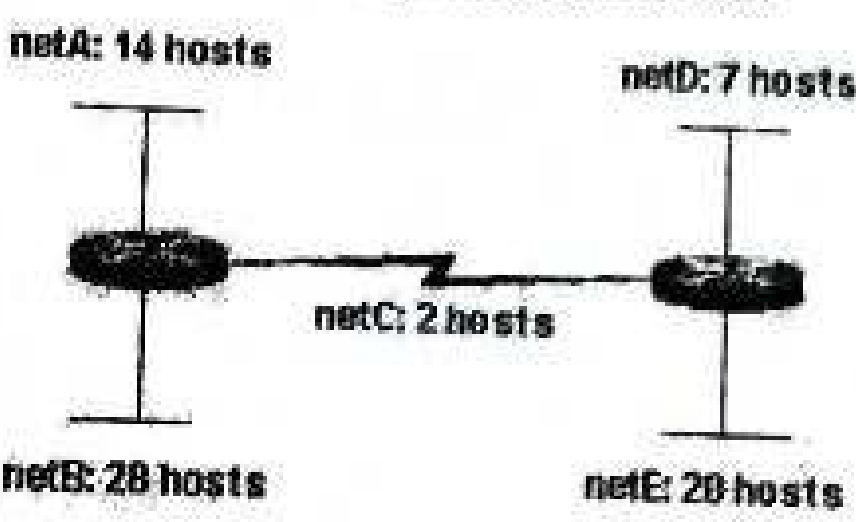
\includegraphics[width=4in]{cn_1}

			\item How can you dedicate 10, 12, 8, 14 public IP address to department A, B, C and D respectively from the pool of class C with minimum losses of IP? Explain. \hfill [8] (\bo{70 Ch})

			\item A large number of consecutive IP addresses are avialable starting at 193.122.2.1. Suppose that four organizations Pulchowk, Thapathali, WRC and ERC request 6000, 2000, 4000 and 2500 address respectively. Design the network and find the first valid IP address, last IP address and mask in w.x.y.z/s notation for each organization. \hfill [8] (\bo{70 Bh})
		\end{enumerate}

	\pagebreak

\section{Transport Layer}
	\begin{center}(5 Hours/8 Marks)\end{center}
	\subsection{The transport service: Services provided to the upper layers}
		\begin{enumerate}[noitemsep, topsep=0pt]
			\item Why do we need a transport layer? \hfill [2] (\texttt{81 Ba})

			\item What are the major task of transport layer? Explain. \hfill [3] (\bo{75 Bh}) [5] (\bo{76 Ch})
		\end{enumerate}

	\subsection{Transport protocols: UDP, TCP}
		\begin{enumerate}[noitemsep, topsep=0pt]
			\item Draw the segment of UDP. \hfill [2] (\texttt{81 Ba})

			\item Define UDP with its header structure. \hfill [4] (73 Ma)

			\item Compare TCP with UDP. \hfill [2] (75 Ba) [3] (75 Ash) [4] (\bo{73 Ch}, \texttt{81 Ba, 80 Ba})

			\item Explain the TCP datagram format in detail. \hfill [5] (75 Ash)

			\item Explain TCP with its Header format. \hfill [6] (75 Ba, 74 Ash)

			\item Explain TCP segment structure. \hfill [4] (\bo{76 Ch}) [6] (\bo{75 Bh})
			\lb Draw the segment structure of TCP and explain briefly. \hfill [5] (\bo{76 Bh})

			\item Explain TCP three way handshaking process. \hfill [4] (\bo{74 Bh})

			\item For client-server application over TCP, why must the server program be executed before the client program? \hfill [3] (\bo{73 Ch})

			\item Why TCP is known as reliable protocol and also describe how reliability is provided by TCP?
			\enter\hfill [4] (\bo{76 Ch}) [5] (\bo{73 Ch})
		\end{enumerate}

	\subsection{Port and Socket}
		\begin{enumerate}[noitemsep, topsep=0pt]
			\item What is port addressing? \hfill [2] (\bo{79 Ch})

			\item What is significance of port address? \hfill [1] (\bo{\texttt{79 Bh}})
			\lb What is the importance of addressing at transport layer? \hfill [2] (76 Ba)

			\item Discuss about different classes of port addresses defined by IANA. \hfill [3] (\bo{\texttt{79 Bh}})

			\item Why port number is used in networking? \hfill [2] (\bo{77 Ch})

			\item How do you implement TCP socket for network communication. Explain  \hfill [6] (\bo{79 Ch})

			\item Differentiate between port and socket. \hfill [2.5] (\bo{74 Bh})

			\item Define socket. \hfill [1] (\bo{73 Bh}, 74 Ash)
			
			\item Explain socket's importance. \hfill [2] (74 Ash)
		\end{enumerate}

	\subsection{Connection establishment, Connection release}
		\begin{enumerate}[noitemsep, topsep=0pt]
			\item Explain the TCP connection establishment, data transfer and connection termination process with necessary diagrams. \hfill [6] (76 Ba)

			\item Explain connection establishment and termination in TCP. \hfill [4] (\bo{75 Ch, 74 Ch})

			\item Explain Connection management of TCP. \hfill [7] (\bo{73 Bh})
		\end{enumerate}

	\subsection{Flow control and buffering}
		\begin{enumerate}[noitemsep, topsep=0pt]
			\item What is congestion? \hfill [1] (\bo{74 Bh})

			\item What are hte techniques for congestion control? \hfill [3] (\bo{74 Bh})

			\item (Assumed) How do you implement packet congestion control for better QoS? \hfill [4] (\texttt{80 Ba})

			\item What are the factors affecting congestion? \hfill [3] (75 Ba)

			\item Explain connection management of TCP with necessary figures. \hfill [6] (\bo{77 Ch})

			\item How is flow control is addressed by TCP? \hfill [3] (\bo{76 Bh})
		\end{enumerate}

	\subsection{Multiplexing and de-multiplexing}
		\begin{enumerate}[noitemsep, topsep=0pt]
			\item Discuss how multiplexing and de-multiplexing is achieved in Transport Layer with examples.
			\enter\hfill [4] (\bo{\texttt{81 Bh}})
		\end{enumerate}

	\subsection{Congestion control algorithm: Token Bucket and Leaky Bucket Transport Layer}
		\begin{enumerate}[noitemsep, topsep=0pt]
			\item What are the factors affecting Congestion? \hfill [3] (75 Ba)

			\item Explain Token Bucket algorithm. \hfill [3] (\bo{76 Ch}) [4] (\bo{74 Ch, 73 Ch, 72 Ch})
			\lb Write short notes on: Token bucket traffic shaping algorithm. \hfill [2] (\texttt{81 Ba}) [3] (\bo{79 Ch})

			\item How can traffic congestion be controlled by token bucket method? \hfill [4] (\bo{\texttt{79 Bh}, 73 Ch}, 73 Ma)

			\item How is token bucket better than leaky bucket in context with packet loss? Explain. \hfill [4] (\bo{\texttt{81 Bh}})

			\item Explain briefly about Leaky-Bucket algorithm. \hfill [4] (\bo{75 Ch})
		\end{enumerate}

	\pagebreak

\section{Application Layer}
	\begin{center}(5 Hours/8 Marks)\end{center}
	\subsection{Web: HTTP and HTTPS}
		\begin{enumerate}[noitemsep, topsep=0pt]
			\item Write short notes on: Web Server \hfill [3] (73 Ma)

			\item Write short notes on: HTTP methods. \hfill [2] (\texttt{81 Ba})

			\item Write short notes on: HTTP. \hfill [2] (\bo{77 Ch}) [3] (73 Ma)

			\item How a request initiated by a HTTP client is served by an HTTP server? \hfill [3](75 Ba)

			\item Explain how HTTPS works? \hfill [2] (75 Ba)

			\item Why is HTTPS not used for all web traffic? \hfill [2] (\bo{\texttt{81 Bh}})
			
			\item What is the difference between HTTP and HTTPS? \hfill [2] (\bo{76 Bh})
		\end{enumerate}

	\subsection{File Transfer: FTP, PuTTY, WinSCP}
		\begin{enumerate}[noitemsep, topsep=0pt]
			\item What is TFTP? \hfill [2] (\bo{76 Ch})
			
			\item How does FTP work? Explain. \hfill [6] (\bo{\texttt{81 Bh}, 75 Bh})
			\lb Write short notes on: FTP server working principle. \hfill [3] (\bo{79 Ch})
			\lb Explain working principle of FTP with data transfer process including proper port connection. Use proper diagram to justify your answer. \hfill [6] (\bo{76 Ch})

			\item (Assumed) How web server communication and file server communication are possible in network. Explain with used protocols. \hfill [6] (75 Ash)
		\end{enumerate}

	\subsection{Electronic Mail: SMTP, POP3, IMAP}
		\begin{enumerate}[noitemsep, topsep=0pt]
			\item Draw the architecture of Email Agent. \hfill [2] (\texttt{81 Ba})

			\item Write short notes on SMTP. \hfill [2] (\bo{77 Ch})

			\item Compare IMAP and SMTP. \hfill [3] (\bo{74 Bh}, 75 Ba)

			\item Write short notes on: SMTP and POP. \hfill [4] (74 Ash)

			\item Compare IMAP and POP3 protocols. \hfill [3] (\bo{\texttt{79 Bh}, 76 Ch, 74 Ch, 73 Bh})

			\item Explain working principle of E-mail system with a proper diagram. \hfill [6] (\texttt{80 Ba})

			\item How can you transfer mail over internet? \hfill [4] (73 Ma)

			\item Which protocols are used in sending and receiving an email? \hfill [3] (73 Ma)
			\lb Illustrate with figures. \hfill [5] (\bo{74 Ch})

			\item What are mail agents? \hfill [4] (\bo{79 Ch})

			\item Discuss functionalities of mail agents. \hfill [4] (\bo{79 Ch})
		\end{enumerate}

	\subsection{DNS}
		\begin{enumerate}[noitemsep, topsep=0pt]
			\item What is DNS? \hfill [1] (\bo{\texttt{79 Bh}, 76 Ch}, 76 Ba, 73 Ma)

			\item Discuss the DNS records. \hfill [2] (74 Ash)

			\item Write short notes on DNS. \hfill [4] (\bo{73 Ch})

			\item Write short notes on: DNS queries. \hfill [4] (\bo{74 Bh})

			\item Explain DNS servers and its query types. \hfill [5] (\bo{73 Bh})

			\item Explain the working principle of DNS with a proper diagram. \hfill [4] (\bo{\texttt{79 Bh}}) [4] (\bo{76 Ch})
			\lb Explain the working of DNS in detail. \hfill [6] (\bo{76 Bh})
			
			\item Why is DNS distributive in nature? \hfill [2] (\texttt{81 Ba})

			\item Explain iterative query and recursive query of DNS with examples and diagrams. \hfill [4] (\texttt{81 Ba}) [5] (76 Ba) [6] (74 Ash)
 
			\item What are the importance of DNS and HTTP(S) while you are browsing any website? \hfill [6] (\bo{75 Ch})

			\item Differentiate HTTP and DNS. \hfill [2.5] (\bo{74 Bh})
		\end{enumerate}

	\subsection{P2P Applications}
	\subsection{Socket Programming}
		\begin{enumerate}[noitemsep, topsep=0pt]
			\item What is port address and socket address? \hfill [2] (\texttt{80 Ba})

			\item Define socket programming. \hfill [2] (75 Ash)
			\lb Write short notes on Socket programming. \hfill [4] (\bo{74 Ch})
		\end{enumerate}

	\subsection{Application server concept proxy caching, Web/Mail/DNS server optimization}
		\begin{enumerate}[noitemsep, topsep=0pt]
			\item Why do we need proxy servers? \hfill [2] (\bo{75 Ch})
			\lb function of proxy server? \hfill [2] (\bo{75 Bh})
		\end{enumerate}

	\subsection{Concept of traffic analyzer: MRTG, PRTG, SNMP, Packet tracer, Wireshark.}
		\begin{enumerate}[noitemsep, topsep=0pt]
			\item Write short notes on: SNMP. \hfill [2] (\bo{77 Ch})

			\item Write short notes on: Packet tracer. \hfill [2] (\bo{77 Ch})
		\end{enumerate}

	\pagebreak

\section{Introduction to IPV6}
	\begin{center}(4 Hours/8 Marks)\end{center}
	\subsection{IPv6- Advantages}
		\begin{enumerate}[noitemsep, topsep=0pt]
			\item List the advantages of IPv6 over IPv4. \hfill [2] (\bo{76 Ch, 76 Bh}) [4] (74 Ash)

			\item What are the factors that lead to deployment of IPv6? \hfill [2] (\bo{\texttt{79 Bh}})

			\item Why the world has decided to migrate to new internet addressing scheme IPV6? \hfill [3] (\bo{73 Ch})

			\item What are the problems of IPv4? \hfill [1] (\bo{77 Ch})

			\item How IPv6 reduce problems of IPv4? \hfill [2] (\bo{77 Ch})

			\item Difference between IPv6 and IPv4. \hfill [4] (\bo{75 Bh}) [6] (73 Ma)

			\item What are the factors that lead to the speedy development of IPv6? \hfill [4] (\bo{74 Ch})
		\end{enumerate}

	\subsection{Packet formats}
		\begin{enumerate}[noitemsep, topsep=0pt]
			\item What are the features of IPv6 header. \hfill [3] (\texttt{80 Ba})
			\lb unique features? \hfill [2] (\bo{79 Ch})

			\item Explain IPV6 with its frame format. \hfill [4] (\bo{74 Bh})

			\item Show IPv6 datagram format. \hfill [2] (75 Ash)

			\item Explain IPV6 Headers with its features. \hfill [2] (73 Ma)

			\item Compare header fields of IPv4 and IPv6. \hfill [4] (75 Ba)

			\item Explain about the process to simplify the writing address of IPV6? \hfill [4] (75 Ba)
		\end{enumerate}

	\subsection{Extension headers}
		\begin{enumerate}[noitemsep, topsep=0pt]
			\item How extension header is used in IPv6? \hfill [3] (\bo{\texttt{81 Bh}})
		\end{enumerate}

	\subsection{Transition from IPv4 to IPv6: Dual stack, Tunneling, Header Translation}
		\begin{enumerate}[noitemsep, topsep=0pt]
			\item Why do we need to migrate the current IPv4 to IPv6 network? \hfill [2] (\bo{79 Ch})

			\item Explain about tunneling in IPv6. \hfill [4] (\bo{75 Bh})

			\item Explain header translation and tunneling approach used for migrating IPV4 and IPV6.
			\enter\hfill [4] (74 Ash)

			\item If there are IPv4 networks in between two IPv6 endpoints, what type of transition strategies will you suggest? Explain with examples and diagrams. \hfill [6] (\texttt{81 Ba})

			\item Define the transition process from IP4 to IP6. \hfill [4] (\bo{74 Ch})

			\item Explain dual stack transition mechanism from IPv4 to IPv6. \hfill [5] (\bo{\texttt{81 Bh}})

			\item List out different strategies to transit from IPv4 to IPv6. \hfill [1] (\bo{77 Ch})

			\item Explain the strategies used for transition from IPv4 to IPv6. \hfill [5] (\texttt{80 Ba})
			\lb Explain briefly about the process involved in transition of IPv4 to v6. \hfill [6] (\bo{\texttt{79 Bh}})
			\lb Explain any one suitable transition approach. \hfill [2] (\bo{77 Ch}) [4] (\bo{79 Ch})
			\lb Explain any two. \hfill [6] (\bo{76 Ch})
			\lb Explain various. \hfill [6] (\bo{76 Bh})

			\item Explain what address family translation means in IPv4/v6 migration process with an apt figure.
			\enter\hfill [5] (\bo{75 Ch})

			\item Which method do you suggest for the migration of IPv4 to IPv6 and why? \hfill [5] (\bo{73 Ch})

			\item ``IPv4 and IPv6 coexistence" what does this mean? \hfill [3] (\bo{76 Ch, 75 Ch, 73 Ch}) 

			\item What methods are used to interoperate IPv6 and IPv4. \hfill [4] (\bo{74 Bh}) [6] (75 Ash)

			\item Explain dual stack approach with an appropriate figure. \hfill [5] (\bo{76 Ch, 73 Ch})
		\end{enumerate}

	\subsection{Multicasting}
		\begin{enumerate}[noitemsep, topsep=0pt]
			\item Discuss any-cast and multi cast addresses in IPv6 with use cases. \hfill [2] (\texttt{81 Ba})
		\end{enumerate}

	\pagebreak

\section{Network Security}
	\begin{center}(7 Hours/16 Marks)\end{center}
	\subsection{Properties of secure communication}
		\begin{enumerate}[noitemsep, topsep=0pt]
			\item What is netowrk security? \hfill [3] (76 Ba)

			\item Why network security is very important? \hfill [2] (\bo{75 Bh})
			
			\item What are the properties of secure communication?
			\enter\hfill [2] (\bo{\texttt{79 Bh}, 76 Ch, 74 Bh, 73 Ch}) [4] (\bo{76 Ch, 76 Bh, 75 Ch}, 74 Ash)

			\item When can you say your network is comprised? And, how is it caused? \hfill [2+2] (\texttt{80 Ba})

			\item What are the different measures we can apply for network security? \hfill [2] (\bo{79 Ch})

			\item Define type of Encryption used in security. \hfill [5] (\bo{74 Ch})

			\item What are the attributes of information security? \hfill [4] (\bo{73 Ch})
		\end{enumerate}

	\subsection{Principles of cryptography: Symmetric Key and Public Key}
		\begin{enumerate}[noitemsep, topsep=0pt]
			\item What do you mean by cryptography? \hfill [2] (\bo{75 Bh}, 73 Ma)

			\item Draw the block diagram of DES algorithm. \hfill [3] (\bo{\texttt{81 Bh}})

			\item Explain the operation of Data Encryption Standard algorithm. \hfill [6] (75 Ba)

			\item Write short notes on: Deffie Hellman Algorithm. \hfill [2] (\bo{\texttt{81 Bh}}) [4] (74 Ash)

			\item How Deffie Hellman algorithm negotiate a shared key between receiver and transmitter. Explain with example. \hfill [6] (73 Ma)

			\item How can you make your network secure using public key cryptography? \hfill [4] (\texttt{80 Ba})

			\item Write short notes on: Symmetric key cryptography. \hfill [4] (\bo{76 Bh, 75 Ch})

			\item Explain the symmetric key and public key cryptography. \hfill [5] (76 Ba)

			\item Compare symmetric key encryption with asymmetric key encryption. \hfill [3] (75 Ba)
		\end{enumerate}

	\subsection{RSA Algorithm}
		\begin{enumerate}[noitemsep, topsep=0pt]
			\item Explain RSA with examples. \hfill [5] (\bo{\texttt{81 Bh}}) [6] (\bo{79 Ch})
			\lb Explain operation of RSA algorithm. \hfill [4 (\bo{73 Ch})] [5] (75 Ba)

			\item Encrypt the plain text ``MACHINE" using RSA algorithm. \hfill [6] (\texttt{81 Ba})
			\lb message ``network". \hfill [6] (75 Ash)
			\lb message ``MISCELLANEOUS" \hfill [6] (\bo{75 Bh})

			\item Encrypt and decrypt the message ``BEIE" using RSA algorithm. \hfill [6] (\bo{\texttt{79 Bh}})
			\lb message ``RANDOM" \hfill [8] (\bo{77 Ch})
			\lb message ``HELLO" \hfill [6] (\bo{76 Ch})
			\lb message ``ROSE" \hfill [6] (\bo{76 Ch})
			\lb message ``BEX" \hfill [6] (\bo{74 Bh})
			\lb message `OIE`" \hfill [7] (\bo{73 Ch})
		\end{enumerate}

	\subsection{Digital Signatures}
		\begin{enumerate}[noitemsep, topsep=0pt]
			\item How does a Digital Signature work? \hfill [2] (\bo{76 Ch})
			
			\item Write short notes on: Digital Signature. \hfill [4] (\bo{75 Ch})

			\item What are digital signatures? \hfill [2] (75 Ba)
		\end{enumerate}

	\subsection{Securing e-mail (PGP)}
		\begin{enumerate}[noitemsep, topsep=0pt]
			\item Write short notes on: PGP. \hfill [2] (\bo{\texttt{81 Bh}}) [3] (\bo{79 Ch})

			\item How PGP can secure email communication? \hfill [3] (\bo{74 Ch})
		\end{enumerate}

	\subsection{Securing TCP connections (SSL)}
	\subsection{Network layer security (IPsec, VPN)}
		\begin{enumerate}[noitemsep, topsep=0pt]
			\item What is IPSEC? \hfill [2] (\texttt{81 Ba})

			\item Write short notes on: VPN. \hfill [2] (\texttt{81 Ba}) [4] (\bo{77 Ch, 76 Bh, 75 Ch})

			\item What is VPN? \hfill [2] (75 Ash)
		\end{enumerate}

	\subsection{Securing wireless LANs (WEP)}
		\begin{enumerate}[noitemsep, topsep=0pt]
			\item Write short notes: WEP. \hfill [4] (76 Ba)
		\end{enumerate}

	\subsection{Firewalls: Application Gateway and Packet Filtering, and IDS}
		\begin{enumerate}[noitemsep, topsep=0pt]
			\item Write short notes on: IDS. \hfill [2] (\texttt{81 Ba})

			\item Write short notes on: Firewall. \hfill [4] (\bo{77 Ch, 74 Bh, 73 Ch})
			\lb Write short notes on: Firewall and types. \hfill [4] (\bo{76 Ch, 74 Ch}, 75 Ba)
			\lb Explain how firewall works. \hfill [4] (\bo{76 Ch})

			\item Explain how Packet filtering firewall works. \hfill [4] (\bo{76 Bh, 75 Ch}, 74 Ash)

			\item Explain different types of firewall that can be used to secure the network. \hfill [6] (\bo{75 Bh})
		\end{enumerate}


\end{document}
